\documentclass[twocolumn, 9pt]{extarticle}
\usepackage[utf8]{inputenc}              % Tipos de caracteres
\usepackage[portuges]{babel}             % Português
\usepackage[a4paper, top=1.2cm, bottom=1.2cm, left=1.2cm, right=1.2cm]{geometry}  % Tipo de papel
\usepackage{color}                       % Para tratamento da cor
\usepackage{graphicx}                    % Para a imagem
\usepackage{amsmath}                     % Para as matematiquices
\usepackage{amssymb}
\setlength{\columnsep}{.7cm}
\usepackage[table,xcdraw]{xcolor}
\usepackage{tikz}
\usetikzlibrary{arrows.meta}
\usepackage{comment}
\usepackage{titling}

\renewenvironment{abstract}
 {\small
  \begin{center}
  \bfseries \abstractname\vspace{-.5em}\vspace{0pt}
  \end{center}
  \list{}{
    \setlength{\leftmargin}{0cm}%
    \setlength{\rightmargin}{\leftmargin}%
  }%
  \item\relax}
 {\endlist}

\renewcommand{\abstractname}{Resumo}
\setlength{\droptitle}{-30pt}

\title{\bf Relatório do Segundo Projeto de IA}
\author{
	80832 Margarida Ferreira
    \and
	81805 Duarte David
    }
\date{\small Dezembro de 2017}


\begin{document} 
\twocolumn[
  \begin{@twocolumnfalse}
    \maketitle
    \begin{abstract}
	\normalsize Testam-se vários métodos de aprendizagem sobre diferentes conjuntos de dados. São realizadas uma classificação sobre um conjunto de palavras, duas regressões sobre conjuntos de pontos 2D e uma aprendizagem por reforço sobre um conjunto de trajetórias sobre um grafo com uma topologia 1D. Os resultados obtidos revelaram-se todos abaixo dos limiares máximos permitidos.\par
    \ \\ 
	\end{abstract}
  \end{@twocolumnfalse}
]

\section{Introdução}
O objetivo do presente trabalho é realizar diversos tipos de aprendizagem automática sobre diversos conjuntos de pontos, de forma a perceber, a um nível introdutório, que técnicas aplicar para diferentes tipos de dados. \par

\section{P1 - Métodos de Classificação}
\subsection{O \textit{Dataset}}
O conjunto de dados consiste num conjunto de palavras, cada uma classificada como \textit{True} ou \textit{False}.\par

\subsection{Seleção das \textit{Features}}
Seja $\Sigma$ o alfabeto onde as palavras estão definidas, e o espaço das \textit{features} $\mathbb{R}^5$ (existem 5 \textit{features} e cada \textit{feature} pertence a $\mathbb{R}$, a extração das \textit{features} é definida por uma função ${f\colon \Sigma ^{*} \setminus \{ \epsilon \} \to \mathbb{R}^5}$, tal que ${f(w) = (x_1, x_2, x_3, x_4, x_5)}$, onde:
\begin{itemize}
\itemsep -0.3em
\item $x_1$ é o comprimento de $w$.
\item $x_2$ é a codificação numérica da primeira letra de $w$.
\item $x_3$ é a codificação numérica da segunda letra de  $w$.
\item $x_4$ é a codificação numérica da penúltima letra $w$.
\item $x_5$ é a codificação numérica da última letra de $w$.
\end{itemize}

A escolha das \textit{features} necessita de satisfazer o requisito de que palavras similares se encontram próximas (por uma dada norma) no espaço das \textit{features}. A similaridade das palavras pode ser morfológica ou semântica. Apenas se faz uma pequena tentativa de respeitar o primeiro caso, uma vez que sequer começar a pensar no segundo se tornaria demasiado complexo. Para tentar respeitar a similaridade morfológica, olhamos para as primeiras e últimas letras de cada palavra (palavras semelhantes podem ter o mesmo radical - ``agir" e ``agente", ou podem acabar da mesma maneira (``inteligente" e ``agente"),  indicando semelhança gramatical). É também considerado o tamanho das palavras.\par

Foram consideradas outras características das palavras, como por exemplo o número de vogais, ou a primeira/última letra ser vogal, mas não produziram resultados melhores nem cumpriam os critérios mencionados acima.\par

\subsection{Método de Classificação}

Utilizando um classificador \textbf{k-vizinhos}, com 3 vizinhos, com as \textit{features} descritas acima, consegue obter-se um \textbf{erro de 0.0}. Também foi testado um classificador de \textbf{árvore de decisão}, mas os resultados ficaram aquém do \textbf{k-vizinhos}, obtendo um erro de $\approx$ 0.017.\par

\section{P2 - Métodos de Regressão}
O objeto de estudo desta parte é a aplicação de métodos de regressão à aprendizagem de funções cujo conjunto de partida e de chegada é $\mathbb{R}$. As funções em causa assemelham-se a funções trigonométricas (ou funções trigonométricas inversas) com ruído.\par

\subsection{Escolha e Avaliação dos Modelos}
Tentou aprender-se a função por 3 modelos diferentes de regressão: \textbf{Regressão Linear}, \textbf{Regressão de Cume com Núcleo} e \textbf{Regressão de Árvore de Decisão}.\par

Os modelos foram avaliados através de \textbf{validação cruzada} para determinar aquele que se ajusta melhor aos dados. Destes três, apenas se observou resultados aceitáveis com a \textbf{Regressão de Cume com Núcleo}.\par

Ajustaram-se dois parâmetros do modelo, $\alpha$ e $\gamma$, correspondentes à largura da penalização e à largura da função de núcleo (uma função de base radial), respetivamente, até se obterem os parâmetros que melhoram a pontuação obtida pela validação cruzada.\par

Para $\alpha = 0.001$ e $\gamma = 0.1$, observou-se uma pontuação de $0.1028$ para a primeira regressão e $547.94$, sendo este o modelo treinado no ficheiro submetido. Também se averiguou que, na segunda regressão, um $\alpha$ arbitrariamente pequeno é aquele que melhora os resultados (uma vez que o \textit{dataset} em questão é muito bem comportado - tem pouco ruído -, não é necessário incluir uma forte penalização pelo sobre-ajustamento). Contudo, valores de $\alpha$ muito pequenos causam o sobre-ajustamento. Os resultados obtidos com estes valores podem ser visualizados na figura 1. As tabelas 1 e 2 mostram as variações das pontuações em função da alteração dos parâmetros.\par
\begin{table}[ht]
\footnotesize
\centering
\begin{tabular}{|rlllll|}
\hline
\multicolumn{1}{|l}{$\gamma$ \textbackslash $\alpha$} & \multicolumn{1}{c}{\textbf{1e-4}} & \multicolumn{1}{c}{\textbf{1e-3}} & \multicolumn{1}{c}{\textbf{1e-2}} & \multicolumn{1}{c}{\textbf{0.1}} & \multicolumn{1}{c|}{\textbf{0.2}} \\ \cline{2-6} 
\multicolumn{1}{|r|}{\textbf{0.01}} & 4.3339 & 3.9898 & 2.1040 & 1.4561 & 1.2814 \\
\multicolumn{1}{|r|}{\textbf{0.05}} & 0.3865 & \cellcolor[HTML]{EFEFEF}\textbf{0.1441} & 0.3435 & 0.6705 & 0.7781 \\
\multicolumn{1}{|r|}{\textbf{0.1}} & 0.3739 & \cellcolor[HTML]{EFEFEF}\textbf{0.1028} & \cellcolor[HTML]{EFEFEF}\textbf{0.1033} & \cellcolor[HTML]{EFEFEF}\textbf{0.2328} & 0.3480 \\
\multicolumn{1}{|r|}{\textbf{0.12}} & 1.7618 & \cellcolor[HTML]{EFEFEF}\textbf{0.0952} & \cellcolor[HTML]{EFEFEF}\textbf{0.1200} & \cellcolor[HTML]{EFEFEF}\textbf{0.2473} & 0.3517 \\
\multicolumn{1}{|r|}{\textbf{0.15}} & 3.5789 & \cellcolor[HTML]{EFEFEF}\textbf{0.2316} & \cellcolor[HTML]{EFEFEF}\textbf{0.1496} & \cellcolor[HTML]{EFEFEF}\textbf{0.2990} & 0.4021 \\
\multicolumn{1}{|r|}{\textbf{0.2}} & 6.3575 & 0.6559 & \cellcolor[HTML]{EFEFEF}\textbf{0.2381} & 0.4000 & 0.5161 \\
\multicolumn{1}{|r|}{\textbf{0.3}} & 9.814 & 1.3326 & 0.4587 & 0.6206 & 0.7636 \\ \hline
\end{tabular}
\caption{\footnotesize Resultados de validação cruzada para o primeiro conjunto de valores. Estão assinalados a sombreado os valores que se encontram dentro dos limites considerados aceitáveis.}
\end{table}
\begin{table}[ht]
\footnotesize
\centering
\begin{tabular}{|rccccc|}
\hline
\multicolumn{1}{|l}{$\gamma$ \textbackslash $\alpha$} & \textbf{1e-5}                           & \textbf{1e-4}                           & \textbf{1e-3}                           & \textbf{1e-2}                           & \textbf{0.1} \\ \cline{2-6} 
\multicolumn{1}{|r|}{\textbf{0.001}}                  & 2428.91                                 & 2988.85                                 & 1621.04                                 & 979.01                                  & 1303.74      \\
\multicolumn{1}{|r|}{\textbf{0.005}}                  & \cellcolor[HTML]{EFEFEF}\textbf{25.39}  & \cellcolor[HTML]{EFEFEF}\textbf{371.58} & 2190.31                                 & 2194.96                                 & 1273.56      \\
\multicolumn{1}{|r|}{\textbf{0.01}}                   & \cellcolor[HTML]{EFEFEF}\textbf{75.43}  & \cellcolor[HTML]{EFEFEF}\textbf{75.79}  & \cellcolor[HTML]{EFEFEF}\textbf{582.05} & 2232.32                                 & 1769.60      \\
\multicolumn{1}{|r|}{\textbf{0.05}}                   & \cellcolor[HTML]{EFEFEF}\textbf{139.11} & \cellcolor[HTML]{EFEFEF}\textbf{154.92} & \cellcolor[HTML]{EFEFEF}\textbf{428.43} & \cellcolor[HTML]{EFEFEF}\textbf{706.73} & 1235.22      \\
\multicolumn{1}{|r|}{\textbf{0.1}}                    & \cellcolor[HTML]{EFEFEF}\textbf{152.89} & \cellcolor[HTML]{EFEFEF}\textbf{308.07} & \cellcolor[HTML]{EFEFEF}\textbf{547.94} & 811.08                                  & 1264.74      \\
\multicolumn{1}{|r|}{\textbf{0.12}}                   & \cellcolor[HTML]{EFEFEF}\textbf{184.63} & \cellcolor[HTML]{EFEFEF}\textbf{329.00} & \cellcolor[HTML]{EFEFEF}\textbf{622.17} & 852.97                                  & 1320.19      \\
\multicolumn{1}{|r|}{\textbf{0.15}}                   & \cellcolor[HTML]{EFEFEF}\textbf{200.70} & \cellcolor[HTML]{EFEFEF}\textbf{434.72} & \cellcolor[HTML]{EFEFEF}\textbf{655.13} & 971.63                                  & 1367.03      \\
\multicolumn{1}{|r|}{\textbf{0.2}}                    & \cellcolor[HTML]{EFEFEF}\textbf{436.47} & \cellcolor[HTML]{EFEFEF}\textbf{532.45} & \cellcolor[HTML]{EFEFEF}\textbf{799.09} & 1103.58                                 & 1445.04      \\
\multicolumn{1}{|r|}{\textbf{0.3}}                    & 1009.01                                 & 910.89                                  & 1043.59                                 & 1305.52                                 & 1601.89      \\ \hline
\end{tabular}
\caption{\footnotesize Resultados de validação cruzada para o segundo conjunto de dados. Estão assinalados a sombreado os valores que se encontram dentro dos limites considerados aceitáveis.}
\end{table}
\begin{figure}[ht]
	\centering
	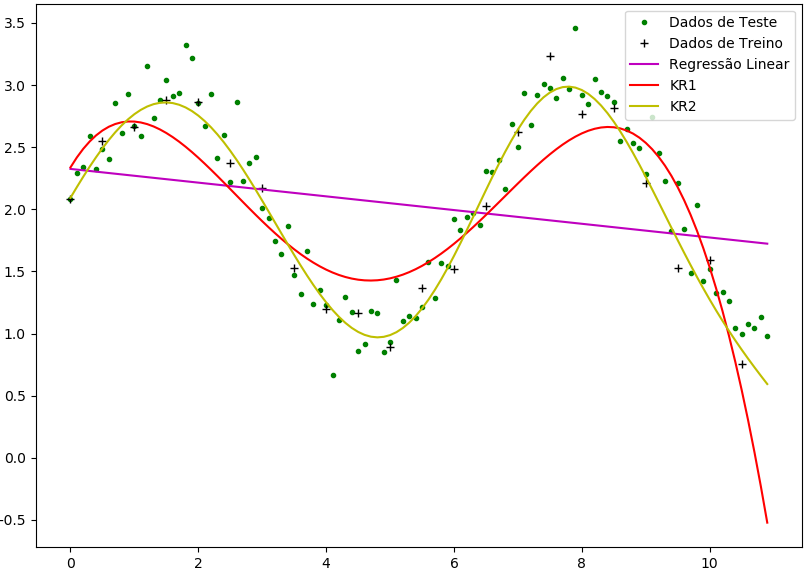
\includegraphics[width=200pt]{Regressoes1.png}
	\par\noindent {\scriptsize a)}
	\\ \
	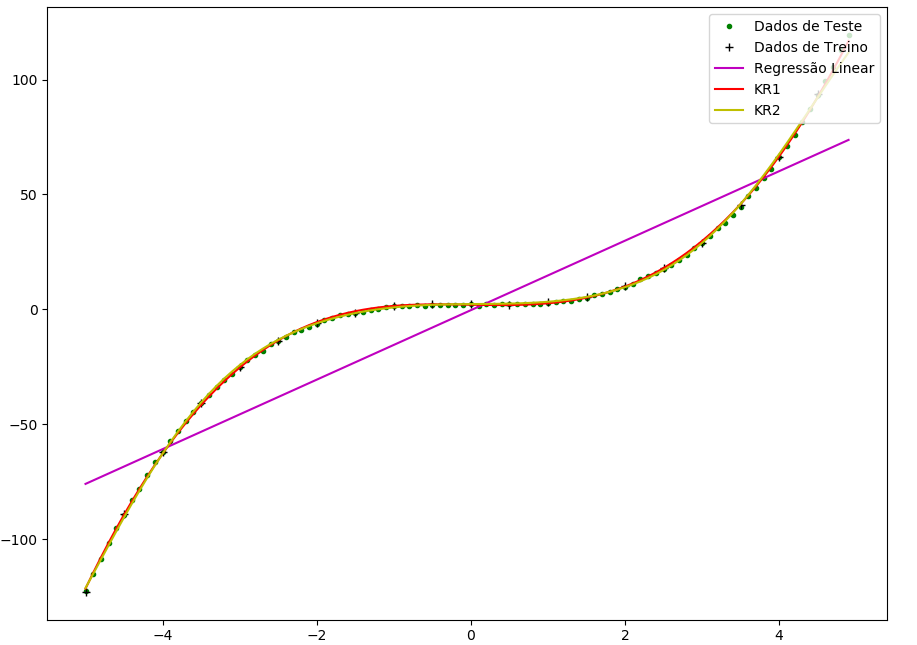
\includegraphics[width=200pt]{Regressoes2.png}
	\par\noindent {\scriptsize b)}
	\caption{\footnotesize Visualização dos dados obtidos para cada uma das regressões, para o primeiro \textit{dataset} (a) e para o segundo (b). KR1 é a Regressão de Cume com Núcleo com $\alpha = 0.00001$ e $\gamma = 0.005$. KR2 é a Regressão de Cume com Núcleo com $\alpha = 0.001$ e $\gamma = 0.1$}
\end{figure}

\section{P3 - Aprendizagem Por Reforço}
O objetivo desta parte é utilizar aprendizagem por reforço para aprender o movimento de um agente num ambiente com 7 estados.\par


\subsection{Política Escolhida}
Uma política é uma função $\pi: S \times A \to [0, 1]$ tal que $\pi(s,a) = P(a_t = a | s_t = s)$, ou seja, é a probabilidade de um agente escolher uma acção com base no estado atual.
A política que escolhemos utiliza o valor da função $Q$ para calcular a probabilidade: é a exponencial de $Q \cdot \eta $ (normalizada tal que $\Sigma_{i=1}^n \pi(s_j,a_i) = 1$, para todo o estado $s_j$), onde $\eta$ é um parâmetro que tem como efeito a separação das probabilidades de cada estado.\par

\subsection{O Ambiente do Agente}
Por inspeção das transições de estados possíveis no primeiro ambiente, obtemos o diagrama de transições que se mostra na figura 2 para o primeiro ambiente. \par
\begin{figure}[ht]
\begin{tikzpicture}
	\definecolor{light-gray}{rgb}{0.9,0.9,0.95}
   
	\node[shape=circle,draw=black, fill=light-gray] (0) at (0, 0) {0};
   	\node[shape=circle,draw=black] (1) at (1.1, 0) {1};
   	\node[shape=circle,draw=black] (2) at (2.2, 0) {2};
    \node[shape=circle,draw=black] (3) at (3.3, 0) {3};
    \node[shape=circle,draw=black] (4) at (4.4, 0) {4};
    \node[shape=circle,draw=black] (5) at (5.5, 0) {5};
    \node[shape=circle,draw=black, fill=light-gray] (6) at (6.6, 0) {6};
	
   	\draw[->, bend left=30] (0) edge node[above] {0} (1);
   	\draw[->, bend left=30] (1) edge node[above] {0} (2);
   	\draw[->, bend left=30] (2) edge node[above] {0} (3);
   	\draw[->, bend left=30] (3) edge node[above] {0} (4);
   	\draw[->, bend left=30] (4) edge node[above] {0} (5);
   	\draw[->, bend left=30] (5) edge node[above] {0} (6);

	\draw[->, loop above] (5) edge node[above] {0} (5);
	\draw[->, loop right] (6) edge node[right] {0} (6);

	\draw[->, bend left=30] (6) edge node[below] {1} (5);
    \draw[->, bend left=30] (5) edge node[below] {1} (4);
    \draw[->, bend left=30] (4) edge node[below] {1} (3);
    \draw[->, bend left=30] (3) edge node[below] {1} (2);
    \draw[->, bend left=30] (2) edge node[below] {1} (1);
    \draw[->, bend left=30] (1) edge node[below] {1} (0);
   
    \draw[->, loop left] (0) edge node[left] {1} (0);
\end{tikzpicture}
\caption{Grafo de transições do agente}
\end{figure}
Cada estado tem no máximo dois estados vizinhos, pelo que se pode pensar num ambiente uni-dimensional para o agente (como por exemplo um braço robótico que apenas rode em um eixo, com travões que o impeçam de dar a volta). Note-se também que a ação 1 aplicada ao estado 5 pode levar ao estado 6 ou a permanecer no estado 5. Conclui-se que o ambiente é estocástico (imagine-se um obstáculo que por vezes impede o braço robótico de rodar).\par
\begin{figure}[ht]
\begin{tikzpicture}
	\definecolor{light-gray}{rgb}{0.9,0.9,0.95}
	
    \node[shape=circle,draw=black, fill=light-gray] (0) at (0, 0) {0};
   	\node[shape=circle,draw=black] (1) at (1.1, 0.5) {1};
   	\node[shape=circle,draw=black] (2) at (2.2, 1.2) {2};
    \node[shape=circle,draw=black] (3) at (3.3, 1.5) {3};
    \node[shape=circle,draw=black] (4) at (4.4, 1.5) {4};
    \node[shape=circle,draw=black] (5) at (5.5, 1.2) {5};
    \node[shape=circle,draw=black, fill=light-gray] (6) at (6.6, .5) {6};
	
   	\draw[->, bend left=30] (0) edge node[above] {0} (1);
   	\draw[->, bend left=30] (1) edge node[above] {0} (2);
   	\draw[->, bend left=30] (2) edge node[above] {0} (3);
   	\draw[->, bend left=30] (3) edge node[above] {0} (4);
   	\draw[->, bend left=30] (4) edge node[above] {0} (5);
   	\draw[->, bend left=30] (5) edge node[above] {0} (6);

	\draw[->, loop above] (5) edge node[above] {0} (5);
	\draw[->, bend left=30] (6) edge node[below] {0} (1);

	\draw[->, bend left=30] (6) edge node[below] {1} (5);
    \draw[->, bend left=30] (5) edge node[below] {1} (4);
    \draw[->, bend left=30] (4) edge node[below] {1} (3);
    \draw[->, bend left=30] (3) edge node[below] {1} (2);
    \draw[->, bend left=30] (2) edge node[below] {1} (1);
    \draw[->, bend left=30] (1) edge node[below] {1} (0);
   
    \draw[->, loop left] (0) edge node[left] {1} (0);
\end{tikzpicture}
\caption{\footnotesize Grafo de transições do agente}
\end{figure}
Na figura 3 mostra-se o diagrama das transições no segundo ambiente, obtido da mesma forma que para o primeiro.\par
Agora, quando é efetuada a ação 0 no estado 6, o estado seguinte é o estado 1. Pode continuar a representar um braço robótico, desta vez sem um dos travões: quando roda mais um pouco (ação 0) após estar orientado para cima (estado 6), ``cai'' para trás e apenas para de rodar ao atingir o estado 1.\par

\subsection{Recompensa}

Em ambos os ambientes, existe uma recompensa de 1 para os estados 0 e 6 (estados objetivo).\par
Esta recompensa será propagada para a função Q ao longo das iterações sucessivas de modo a que o agente aprenda a escolher transições que o levem a estes estados o mais depressa possível. Isto reflete-se na função da política, cuja probabilidade de escolher uma ação cresce exponencialmente com o valor Q associado a essa transição.\par

\subsection{Resultado}
Foi aplicado o algoritmo \textit{Q-learning} para diferentes valores de $\alpha$ e $\gamma$. Com valores de $\alpha$ elevados, o algoritmo consegue convergir rapidamente, pelo que se conclui que os ambientes são pouco estocásticos. Para valores $\alpha$ menores, o algoritmo obtém valores com erro inferior, a custo de mais iterações. Para contornar este problema, decrementa-se o valor de $\alpha$ a cada iteração do algoritmo.\par
Assim, foram escolhidos os valores ${\alpha_{inicial} = 0.5}$ e ${\gamma = 0.9}$ e usado para cada iteração $i$ o valor ${\alpha = \frac{5}{5+i} \cdot \alpha_{inicial}}$, por apresentarem os erros mais baixos ($\approx 0.09$ para ambos os ambientes).\par
Com estes valores, ao ser colocado no estado 5 do primeiro ambiente, o agente exerce a ação 0, apesar do elemento estocástico da mesma, com o intuito de se colocar no estado 6, no qual permanece (recebendo uma recompensa de 1 em cada \textit{time step}. No segundo ambiente, como não é possível permanecer no estado 6, o agente desloca-se com a intenção de alcançar o estado 0, através dos estados 6 e 1\par
Por outro lado, ao ser colocado no estado 3, o agente opta por se deslocar para o estado 0, em ambos os ambientes, e manter-se lá. Esta preferência pelo estado 0 em detrimento do estado 6 (ambos à mesma distância do 3) resulta da tendência do agente a evitar movimentos incertos, como aquele com que se depararia ao tentar deslocar-se do estado 5 para o 6.\par

\section{Conclusão}
Foram realizados com sucesso diversos tipos de aprendizagem automática. Observou-se as implicações que os parâmetros de cada um dos métodos têm e cumpriu-se o objetivo de perceber como analisar os dados, tomando especial cuidado para evitar que os métodos se sobre-ajustem aos dados.\par
\end{document}
